\title{%
  Conclusions of the course
}
\author{Daniel Bosk}
\institute{%
  MIUN IST
}

\mode<article>{\maketitle}
\mode<presentation>{%
  \begin{frame}
    \maketitle
  \end{frame}
}

\mode*

\begin{abstract}
  \mode*

% What's the problem?
% Why is it a problem? Research gap left by other approaches?
% Why is it important? Why care?
% What's the approach? How to solve the problem?
% What's the findings? How was it evaluated, what are the results, limitations, 
% what remains to be done?

% XXX Summary
\emph{Summary:}
In this learning session we will cover the foundations of security.
By this we mean what security is all about, \eg what types of properties we are 
interested in and what we want to achieve in our security work.
We will also introduce the scientific method and, particularly, how this can be 
applied in the area of security to create new knowledge.

Finally, we will cover usability and how users' weaknesses affects security.
There are many ways to attack systems through their human operators.
We must consider usability when designing secure systems.

% XXX Motivation and intended learning outcomes
\emph{Intended learning outcomes:}
After this session you should be able:
\begin{itemize}
  \item to \emph{understand} the what security is generally about.
  \item to \emph{differentiate} which types of scientific methods are 
    appropriate to answer a given question.
  \item to \emph{adopt} an adversarial thinking for situtions involving humans.
  \item to \emph{incorporate} basic psychology in the design of a system to 
    increase its security.
\end{itemize}

% XXX Prerequisites
%\emph{Prerequisites:}
%\dots

% XXX Reading material
\emph{Reading:}
You should read Gollmann's chapter on \enquote{Foundations of Computer 
  Security}~\cite[Chap.\ 3]{Gollmann2011cs}.
There he attempts at a definition of Computer Security and related terms, \eg 
confidentiality, integrity, and availability, which we need for our treatment of 
the topic.
Anderson also covers this in Chapter 1 of~\cite{Anderson2008sea}.
He also treats a wider area than just \emph{computer} security, which is good 
for us, he covers many aspects of security in different examples.

For the introduction to the scientific method you should read 
\citetitle{HowToDesignSecurityExperiments}~\cite{HowToDesignSecurityExperiments}.
This paper discusses the scientific method of (parts of) the security field.
For a more in-depth reflection on the state of security as a scientific pursuit, 
we recommend
\citetitle{SecurityAsAScience}~\cite{SecurityAsAScience}.

\Citeauthor{Anderson2008sea} gives a short summary of the psychology of users, 
their strengths and weaknesses, and how usability affects security in Chapter 2 
\enquote{Usability and Psychology} of 
\citetitle{Anderson2008sea}~\cite{Anderson2008sea}.

\end{abstract}


\section{What were the core things?}

\subsection{Foundations}

\begin{frame}
  \begin{itemize}
    \item What is security?
    \item The scientific method
    \item Security usability
  \end{itemize}
\end{frame}

\begin{frame}
  \begin{block}{Security}
    \begin{itemize}
      \item Policy (goals)
      \item Enforcement through mechanisms.

        \pause

      \item System model
      \item Adversary model
    \end{itemize}
  \end{block}
\end{frame}

\begin{frame}
  \begin{block}{Scientific method}
    \begin{itemize}
      \item Inductive (experiments)
      \item Deductive (proofs)
      \item Quantitative (statistics)
      \item Qualitative (details of why)
    \end{itemize}
  \end{block}
\end{frame}

\begin{frame}
  \begin{block}{Usability}
    \begin{itemize}
      \item If you don't give your users usability, you make them your enemy.
    \end{itemize}
  \end{block}
\end{frame}

\subsection{Info theory and crypto}

\begin{frame}
  \begin{itemize}
    \item Information theory
    \item Cryptography
  \end{itemize}
\end{frame}

\begin{frame}
  \begin{block}{Info theory}
    \begin{itemize}
      \item Entropy (measure unpredictability)
    \end{itemize}
  \end{block}

  \begin{example}
    \begin{itemize}
      \item Gussability for passwords
      \item Identifiability of users (tracking)
    \end{itemize}
  \end{example}
\end{frame}

\begin{frame}
  \begin{block}{Crypto}
    \begin{itemize}
      \item Shared-key encryption
      \item One-way functions and message authentication

        \pause

      \item Key exchange
      \item Public-key encryption
      \item Digital signatures

        \pause

      \item Secure multiparty computation
      \item Zero-knowledge proofs-of-knowledge
    \end{itemize}
  \end{block}
\end{frame}

\subsection{Authentication}

\begin{frame}
  \begin{itemize}
    \item Bootstrapping authentication
    \item User-to-machine authentication
    \item Something-you-know (passwords)
    \item Something-you-have (HW, keys?)
    \item Machine-to-user authentication
  \end{itemize}
\end{frame}

\subsection{Protocols}

\begin{frame}
  \begin{itemize}
    \item What's a protocol? (Putting things together)
    \item Modelling protocols to analyse security properties
    \item Cheating on an exam
    \item Stealing a Tesla
    \item Challenge--response
  \end{itemize}
\end{frame}

\subsection{Access control}

\begin{frame}
  \begin{itemize}
    \item Access control models
    \item Multi-level security
    \item Multi-lateral security
  \end{itemize}
\end{frame}

\subsection{Accountability}

\begin{frame}
  \begin{itemize}
    \item Book-keeping
    \item Clark-Wilson security policy model
    \item Logging
    \item DLTs
  \end{itemize}
\end{frame}

\subsection{Trusted computing}

\begin{frame}
  \begin{itemize}
    \item DRM
    \item Root of trust
    \item Secure enclaves (SGX)
    \item Trusted computing
    \item Side channels
    \item Digital rights management (DRM hackathon)
  \end{itemize}
\end{frame}

\subsection{Software security}

\begin{frame}
  \begin{itemize}
    \item Smashing the stack \etc
  \end{itemize}
\end{frame}


\section{Exercise}

\subsection{From the news}

\begin{frame}
  \begin{figure}
    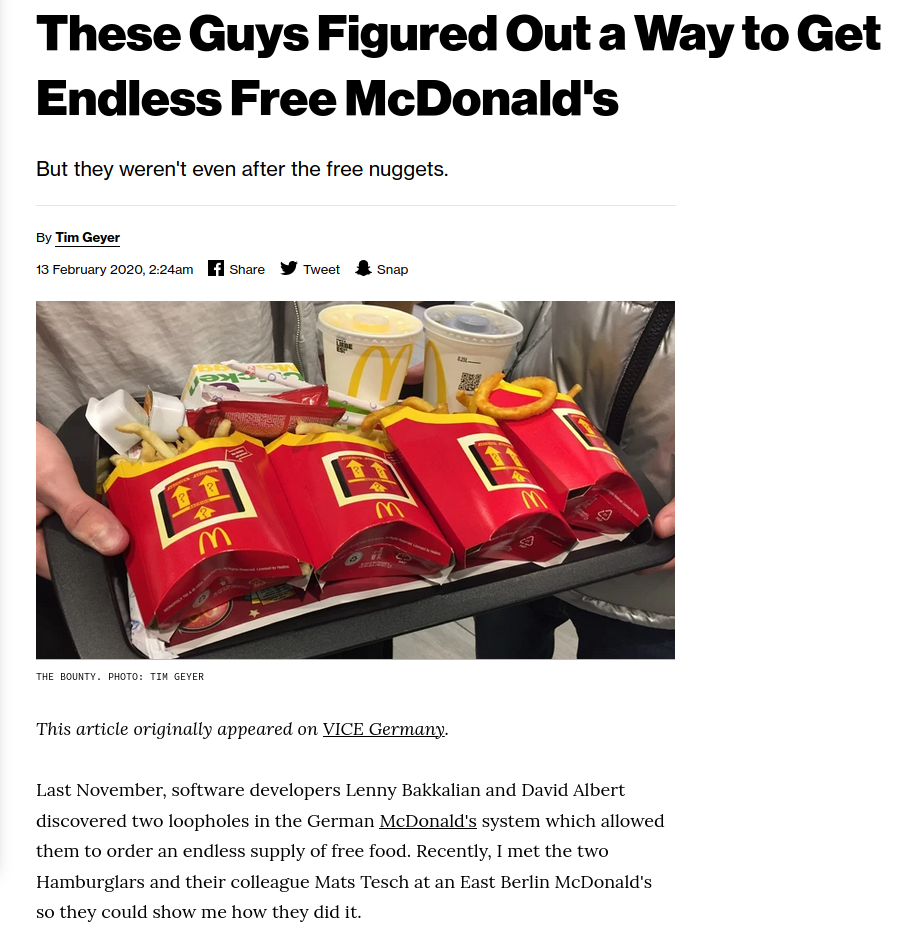
\includegraphics[height=0.8\textheight]{McDo-heist.png}
  \end{figure}
  \url{https://www.vice.com/en_au/article/4agvdw/mcdonalds-hack-free-food}
\end{frame}

\subsection{Proper security for food app}

\begin{frame}
  \begin{exercise}[Design app]
    \begin{itemize}
      \item Order food
      \item Pick-up food
      \item Discount coupons
    \end{itemize}
  \end{exercise}
\end{frame}

\section{The exam}

\mode<all>{\endinput}

\subsection{The rules}

\begin{frame}
  \begin{itemize}
    \item Motivate your answers.
    \item Lack of motivation yields zero points.
  \end{itemize}
\end{frame}

\begin{frame}
  \begin{description}
    \item[Time] 5 hours.
    \item[Aids] Dictionary.
  \end{description}
\end{frame}

\begin{frame}
  \begin{itemize}
    \item Each question can be awarded up to three points:
      \begin{description}
        \item[1p] E
        \item[2p] C
        \item[3p] A
      \end{description}
    \item E on the exam: you must get at least one point on each question.
    \item D on the exam: you're more than halfway to C.
    \item C on the exam: you must get at least two points on each question.
    \item B on the exam: you're more than halfway to A.
    \item A on the exam: you must get three points on each question.
  \end{itemize}
\end{frame}

\subsection{Some questions}

\begin{frame}
  \begin{exercise}
    Describe the terms
    \begin{enumerate}
      \item identification and
      \item authentication.
    \end{enumerate}
    Make sure to illustrate your explanations by examples.
    You must also give an example of a mechanism for each of the terms.
  \end{exercise}
\end{frame}

\begin{frame}
  \begin{solution}
    In identification you claim an identity.
    This can be done using e.g.~a username, fingerprint or DNA sequence.

    In authentication you prove you are who you claim you are.
    This can be done using e.g.~\emph{who} you are (biometric), \emph{where} 
    you are (location) or what you \emph{do} (biometric), something you 
    \emph{have} (e.g.~BankID), or something you \emph{know} (password).
  \end{solution}
\end{frame}


\begin{frame}
  \begin{exercise}
    Separation of duties is a core concept for security.
    \begin{enumerate}
      \item Describe the two types of separation of duties.
      \item What is the main reason for separation of duties?
    \end{enumerate}
  \end{exercise}
\end{frame}

\begin{frame}
  \begin{solution}
    There are two types of separation of duties:
    dual control and functional separation.
    Dual control means that two or more subjects must act together (at the same 
    time) to authorize a transaction.
    Functional separation means that several functions are needed to authorize 
    a transaction---e.g.~create a transaction and verify it---and one subject 
    is not allowed to do both functions.

    The reason for separation of duties to make it impossible for one malicious 
    subject to compromise a system.
    With separation of duties the malicious subject must persuade one or more 
    other subjects to collude.
  \end{solution}
\end{frame}

  
\begin{frame}
  \begin{exercise}
    Give an example of a passive side-channel attack.
  \end{exercise}
\end{frame}

\begin{frame}
  \begin{solution}
    The adversary is interested in learning classified information.
    They set up a device which records electromagnetic emissions to reconstruct 
    the image on a screen, thus when a target works with the classified data on 
    the computer the adversary sees the same image.
    This is a passive attack since we only need to record.
  \end{solution}
\end{frame}


\begin{frame}
  \begin{exercise}
    There are three approaches to security: prevention, detection and reaction.
    Discuss why security is not all about prevention, how do the three approaches 
    complement each other.
  \end{exercise}
\end{frame}

\begin{frame}
  \begin{solution}
    The reason for having these three approaches is partly economy and partly 
    that it is impossible to do prevention for certain things.
    Thus, if we cannot prevent an attack, we must be able to detect it.
    When we have detected it we must be able to recover.

    In some cases it's impossible to recover, however.
    For instance, if the attacker gets the personal data of clients.
    We simply cannot take back this data, there will always be a copy somewhere.
    Thus prevention is the main approach for protecting personal data.
    Prevention in this case comes both in terms of protecting the stored data, 
    but also through data minimization, i.e.\ storing only the necessary data, 
    nothing more.

    In other cases, the recovery might be in terms of insurance paying for the 
    costs of the damage, e.g.\ financial loss.

    In some cases, prevention is possible, but detection and recovery is 
    cheaper.
    For instance, the lunch coupons for restaurants can easily be frauded.
    But this will also be easily detectable, thus the cost of prevention might 
    be higher than the cost of the fraud before detection.

    In other cases, e.g.\ electronic communication, then prevention is cheap --- 
    simply use encryption --- whereas detecting a passive eavesdropper is 
    impossible.
  \end{solution}
\end{frame}


\begin{frame}
  \begin{exercise}
    A user wishes to provide confidentiality to a file.
    \begin{enumerate}
      \item She can accomplish this through mechanisms provided in the operating 
        system.
        Explain how this works and what are the limits.

      \item She can also accomplish this through purely cryptographic mechanisms.
        Explain how this works and what are the limits.
    \end{enumerate}
  \end{exercise}
\end{frame}

\begin{frame}
  \begin{solution}
    The first way she's securing her file is by using access control mechanisms 
    in the operating system (OS).

    Assuming we have physical access to the computer, then we can just read the 
    raw data from the disk.
    This can be accomplished by either booting our own OS on her computer, or 
    by removing the disk.

    If we don't have physical access we can always try to bypass the access 
    control mechanisms in other ways, e.g.\ by gaining privileges in the system 
    or seeing if the OS has failed to protect reading from the raw disk (i.e.\ 
    not using the file system).

    The main point here is that the operating system must be working correctly 
    for its mechanisms to be effective.
    The \emph{running} operating system will provide confidentiality by not 
    allowing other users' requests to open the file.

    The most obvious way to have system independent security for this file is 
    to encrypt it, i.e.~using cryptographic mechanisms.
    This way no one can read it unless they have access to the key, and this is 
    true no matter if you change the environment.
    (Of course, if the system is untrusted someone can get to the key that way, 
    but that's outside the scope of this question.)
  \end{solution}
\end{frame}


  
\begin{frame}
  \begin{exercise}
    Can files such as images (e.g.\ JPEGs) and other data be dangerous?
  \end{exercise}
\end{frame}

\begin{frame}
  \begin{solution}
    Yes, they can contain machine code which can be executed if there is e.g.\ 
    a buffer overrun vulnerability in the software that reads the data.
  \end{solution}
\end{frame}



\begin{frame}
  \begin{exercise}
    You want to develop a competitor to the major streaming services.
    You want to provide a privacy-preserving service which follows age limits 
    (parental guidance).
    How would you go about to implement it?
  \end{exercise}
\end{frame}

\begin{frame}
  \begin{solution}
    Anonymous credentials based on zero-knowledge proofs of knowledge.
  \end{solution}
\end{frame}


